\chapter{KAJIAN PUSTAKA}

\section{Penelitian Terdahulu}

Pengembangan sistem \textit{Graph-RAG} akademik mengandalkan integrasi antara ekstraksi informasi terstruktur dan mekanisme pencarian hibrida. Rangkuman studi yang menjadi acuan teknis dalam penelitian ini disajikan pada ~\ref{tab:penelitian_terdahulu_revisi}.

\renewcommand{\arraystretch}{1.3} % Memberi jarak vertikal antar baris
\begin{longtable}{|p{3cm}|p{2cm}|p{5cm}|}
    \caption{Tinjauan Penelitian Terdahulu} \label{tab:penelitian_terdahulu_revisi} \\
    
    \hline
    \textbf{Judul} & \textbf{Penulis} & \textbf{Kesimpulan} \\ \hline
    \endfirsthead

    \hline
    \textbf{Judul} & \textbf{Penulis} & \textbf{Kesimpulan} \\ \hline
    \endhead

    \hline
    \multicolumn{3}{r}{\textit{Bersambung ke halaman berikutnya...}} \\
    \endfoot

    \hline
    \endlastfoot

    % --- Studi 1 (Sudah Benar) ---
    \textit{Knowledge Graph Generation and Application for Unstructured Data Using Data Processing Pipeline} &
    \cite{thushara2024} &
    Penggunaan model generatif \textit{REBEL} dalam \textit{pipeline} NLP modular terbukti sangat efektif untuk konstruksi \textit{Knowledge Graph} otomatis dengan akurasi 87\%. Metode ini bekerja 3x lebih cepat dibandingkan teknik tradisional dalam mengekstraksi relasi dari teks tidak terstruktur.
    \\ \hline

    % --- Studi 2 (Diperbaiki) ---
    \textit{HybridRAG: Integrating Knowledge Graphs and Vector Retrieval Augmented Generation for Efficient Information Extraction} & 
    \cite{10.1145/3677052.3698671} & 
    Integrasi sistematis antara jalur vektor dan graf (\textit{HybridRAG}) menghasilkan performa paling seimbang dengan skor \textit{Faithfulness} dan \textit{Answer Relevancy} sebesar 0,96. \textit{GraphRAG} unggul dalam menjawab pertanyaan faktual, sementara \textit{VectorRAG} lebih efektif untuk pertanyaan abstraktif.
    \\ \hline

    % --- Studi 3 (Diperbaiki) ---
    \textit{Open-Source Agentic Hybrid RAG Framework for Scientific Literature Review} & 
    \cite{nagori2025opensourceagentichybridrag} & 
    Kerangka kerja \textit{Agentic Hybrid RAG} memungkinkan agen otonom untuk secara dinamis memilih jalur \textit{retrieval} terbaik (Graf atau Vektor) berdasarkan karakteristik kueri. Pendekatan ini meningkatkan relevansi jawaban, memitigasi halusinasi, dan menyertakan estimasi ketidakpastian (\textit{uncertainty}).
    \\ \hline
\end{longtable}

\section{Kajian Teori}

\subsection{Scholarly Search}

Saat ini, sistem pencarian ilmiah sering menghadapi tantangan berupa fragmentasi data, di mana informasi penting tersebar di berbagai platform yang tidak saling terhubung. Untuk mengatasi permasalahan ini, telah dikembangkan berbagai sistem pencarian akademik seperti \textit{Google Scholar}, \textit{Semantic Scholar}, \textit{AMiner}, \textit{Microsoft Academic Search}, dan \textit{CiteSeerX}. Di antara platform-platform tersebut, \textit{Google Scholar} memiliki cakupan literatur yang paling luas \citep{10.1007/s11192-020-03690-4}. Namun, masalahnya adalah bahwa Google Scholar dan solusi serupa lainnya sangat bergantung pada jumlah sitasi untuk memberi peringkat pada daftar kandidat artikel yang relevan. Ketika mekanisme pemeringkatan ini kurang efektif, pengguna cenderung beralih ke platform pencarian lain sepert \textit{PubMed}, \textit{Microsoft Academic Search}, atau \textit{Semantic Scholar}. Platform-platform alternatif tersebut mengadopsi berbagai teknik analitik untuk meningkatkan kualitas hasil pencarian, termasuk pengukuran tingkat pengaruh publikasi \citep{Shen2016ModelingTA}.

Tantangan penelitian yang paling mendesak dalam bidang ini adalah bagaimana mendefinisikan serta mengukur kesamaan (\textit{similarity}) dan relevansi semantik antar artikel secara akurat. Beberapa pendekatan sebelumnya mencoba mengatasi hal ini dengan memanfaatkan informasi tekstual dan struktural. Oleh karena itu, diperlukan representasi data berbasis graf yang mampu mengintegrasikan data \textit{heterogen} tersebut guna mendukung penemuan pengetahuan (\textit{knowledge discovery}) yang lebih efisien. Contohnya, studi dari \cite{DBLP:conf/semweb/MaiJY18} mengadopsi penggunaan \textit{embeddings} tekstual dan struktural untuk menemukan makalah yang relevan dengan kueri. Namun, pendekatan-pendekatan tersebut umumnya menggunakan \textit{supervised learning} yang memerlukan data pelatihan berlabel dan penyetelan parameter dalam pengambilan literatur. Hal ini berbeda dengan pendekatan yang diusulkan dalam penelitian ini, yang menitikberatkan pada metode \textit{unsupervised} atau \textit{zero-shot}.

\subsection{Knowledge Extraction}
Secara teoretis, \textit{Information Extraction} (IE) merupakan proses dalam \textit{Natural Language Processing} (NLP) yang bertujuan mengekstraksi pengetahuan terstruktur dari teks tidak terstruktur \citep{WANG2018112}. Namun, dalam arsitektur \textit{Graph-RAG}, menurut \cite{mondal2021end}, proses ini secara spesifik diwujudkan sebagai \textit{Knowledge Extraction} (KE), yaitu fase dimana untuk mengonversi informasi mentah menjadi format data terstruktur melalui pengenalan entitas dan ekstraksi relasi. Implementasi \textit{Knowledge Extraction} berfungsi sebagai fondasi untuk membangun basis pengetahuan (\textit{knowledge base}) yang dapat memfasilitasi mekanisme penalaran sistem dalam menghasilkan jawaban yang akurat.

Secara formal, tugas \textit{Knowledge Extraction} dapat diformulasikan sebagai fungsi pemetaan dari teks input \(\mathcal{T}\) menjadi representasi terstruktur \(\mathcal{S}\). Representasi ini terdiri dari himpunan entitas \(E\) dan relasi \(R\), sebagaimana dinyatakan dalam Persamaan \ref{eq:ie-mapping}:

\begin{equation}
\mathcal{S} = f_{IE}(\mathcal{T}) = \{(e_i, r_{ij}, e_j) \mid e_i, e_j \in E, r_{ij} \in R\}
\label{eq:ie-mapping}
\end{equation}

\noindent di mana setiap elemen dalam \(\mathcal{S}\) berupa \textit{triplet} \((e_i, r_{ij}, e_j)\) yang merepresentasikan satu fakta tunggal, dengan \(e_i\) bertindak sebagai entitas subjek, \(r_{ij}\) sebagai predikat atau relasi, dan \(e_j\) sebagai entitas objek.

Guna mengimplementasikan fungsi pemetaan tersebut pada data berskala besar, diperlukan pendekatan otomatisasi. \cite{Premasiri2025} menyoroti bahwa skalabilitas ekstraksi manual tidak lagi memadai untuk menangani volume data tekstual yang terus berkembang. Oleh karena itu, otomasi IE menjadi esensial untuk mentransformasi teks menjadi \textit{structured knowledge} secara efisien. Agar proses ekstraksi berjalan sistematis, \textit{Knowledge Extraction} umumnya didekomposisi menjadi tiga tahapan fundamental sebagai berikut:

\begin{enumerate}[label=\textbf{\arabic*.}, leftmargin=*, itemsep=10pt]
    \item \textbf{\textit{Named Entity Recognition} (NER)}
    
    \hspace*{0.75cm} Sebagai langkah awal dalam \textit{pipeline}, \textit{Named Entity Recognition} (NER) bertugas mengidentifikasi dan mengklasifikasikan entitas penting yang terdapat dalam teks. Proses ini berkaitan langsung dengan penemuan himpunan entitas \(E\) pada Persamaan \ref{eq:ie-mapping}. NER mendeteksi istilah relevan—seperti nama orang, organisasi, lokasi, atau terminologi ilmiah—dan memberikan label kategori yang sesuai \cite{ZHAO2023225}.

    \item \textbf{\textit{Relation Extraction} (RE)}
    
    \hspace*{0.75cm} Setelah entitas berhasil diidentifikasi, tahap berikutnya adalah \textit{Relation Extraction} (RE). Tugas ini bertujuan menemukan \(r_{ij}\) yang menghubungkan dua entitas (\(e_i\) dan \(e_j\)) secara semantik. RE mengklasifikasikan jenis hubungan yang terjadi, misalnya hubungan ``menggunakan'' dalam kalimat ``Metode A menggunakan Algoritma B'', atau hubungan ``dikembangkan oleh'' pada sitasi penulis.

    \item \textbf{\textit{Event Extraction} (EE)}
    
    \hspace*{0.75cm} Untuk memperkaya lapisan semantik, IE sering kali dilengkapi dengan \textit{Event Extraction}. Berbeda dengan RE yang memetakan hubungan statis, EE bertujuan mengidentifikasi peristiwa dinamis yang mencakup pemicu kejadian (\textit{trigger}) serta argumen pendukungnya (pelaku, waktu, lokasi, dan hasil).
    
\end{enumerate}

Dalam konteks penelitian ini, prinsip-prinsip \textit{Knowledge Extraction} tersebut diimplementasikan secara spesifik untuk menstrukturisasi domain literatur akademik. Sebagaimana didemonstrasikan oleh \cite{GAJENDRAN2023107808}, integrasi \textit{NER} dan \textit{RE} mampu mentransformasi data tekstual menjadi \textit{Knowledge Graph} yang koheren dalam basis data graf seperti \textit{Neo4j}. Guna menangani kompleksitas terminologi ilmiah yang rumit, pendekatannya mulai beralih dari metode konvensional menuju model \textit{Deep Learning} berbasis \textit{Transformers} seperti \textit{BERT} (\cite{jain-etal-2020-scirex}) atau \textit{SciBERT} \citep{beltagy-etal-2019-scibert}yang terbukti unggul dalam menangkap konteks semantik. Dengan demikian, arsitektur \textit{KE} dalam penelitian ini berfungsi sebagai komponen vital yang mengonversi abstrak publikasi menjadi \textit{triplet} pengetahuan \((subject, predicate, object)\), yang selanjutnya diintegrasikan menjadi struktur graf komprehensif untuk mendukung pencarian referensi yang relevan.

\subsection{Knowledge Graph}

Secara umum, basis pengetahuan (\textit{knowledge base}) adalah kumpulan data yang menggambarkan fakta dunia nyata dan hubungan maknanya dalam bentuk \textit{triplet}. Ketika kumpulan \textit{triplet} tersebut direpresentasikan dalam bentuk jaringan—di mana entitas menjadi titik (\textit{node}) dan hubungannya menjadi garis (\textit{edge})—maka ia disebut sebagai \textit{Knowledge Graph} (KG) \citep{mondal2021end}. Dalam praktiknya, istilah basis pengetahuan dan \textit{knowledge graph} sering kali dianggap sebagai konsep yang sama dan digunakan secara bergantian.

Secara matematis, \textit{Knowledge Graph} dimodelkan sebagai sebuah graf berarah yang dapat didefinisikan melalui Persamaan \ref{eq:kg-definition}:

\begin{equation}
G = (E, R, T)
\label{eq:kg-definition}
\end{equation}

\noindent Di mana $E$ mewakili himpunan entitas (seperti individu atau konsep), $R$ mewakili himpunan relasi (seperti ``bagian\_dari''), dan $T$ merupakan himpunan \textit{triplet} yang membentuk keseluruhan struktur graf tersebut \cite{Hogan_2021}. Setiap elemen di dalam $T$ merepresentasikan satu fakta tunggal yang diformulasikan sebagai berikut:

\begin{equation}
(h, r, t) \in T
\label{eq:triplet-format}
\end{equation}

\noindent Dalam format ini, entitas asal atau \textit{head} ($h$) terhubung ke entitas tujuan atau \textit{tail} ($t$) melalui suatu relasi ($r$) tertentu \cite{peng2023knowledge}. Sebagai contoh, \textit{triplet} (Jakarta, \textit{capitalOf}, Indonesia) secara otomatis menyimpan pengetahuan bahwa Jakarta adalah ibu kota dari Indonesia. Struktur ini sangat efektif karena arah tautan memberikan makna yang jelas; entitas \textit{head} menunjuk langsung ke entitas \textit{tail} melalui garis relasi (\textit{edge}), sebagaimana dapat dilihat pada Gambar \ref{fig:simple-kg}.

\begin{figure}[htbp]
    \centering
    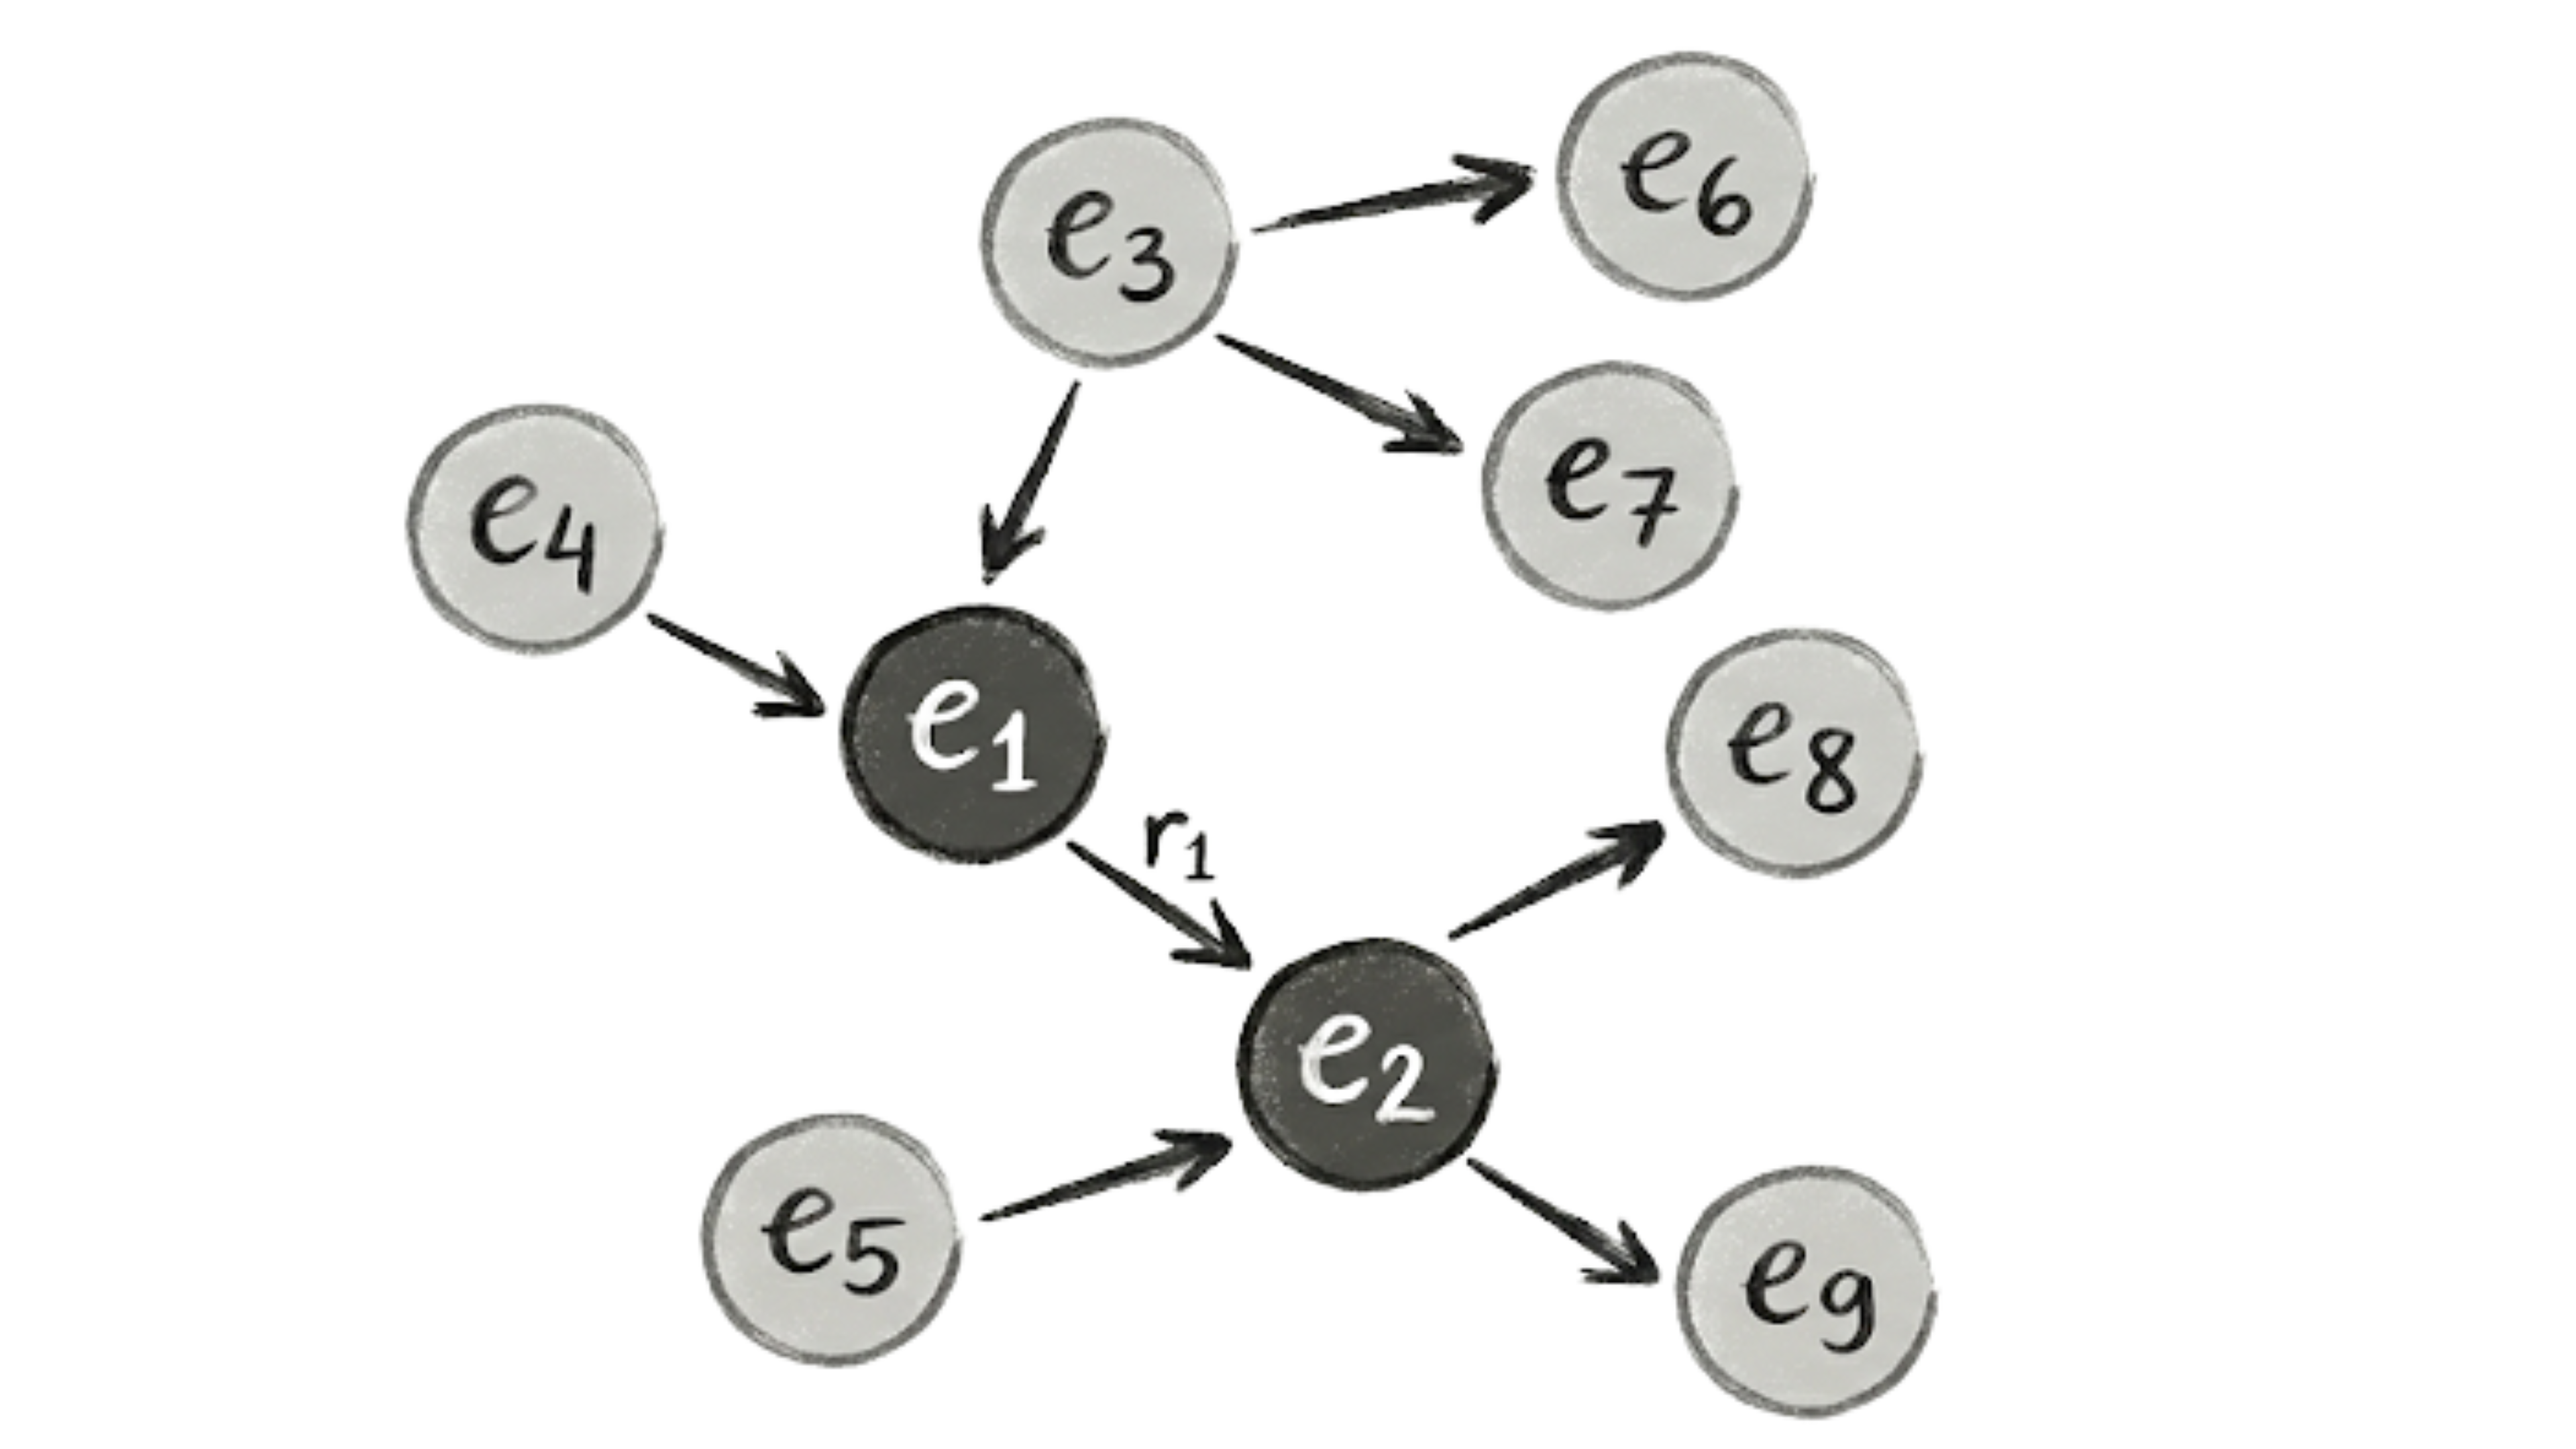
\includegraphics[width=0.8\textwidth]{Gambar/node.png}
    \caption{Contoh sederhana dari \textit{knowledge graph}.}
    \label{fig:simple-kg}
\end{figure}

Ilustrasi pada Gambar \ref{fig:simple-kg} menunjukkan contoh graf pengetahuan sederhana. Sebagaimana terlihat pada gambar tersebut, \textit{node} $e_1$ dan $e_2$ terhubung oleh relasi $r_1$ yang mengarah dari $e_1$ ke $e_2$. Dengan demikian, $e_1, e_2,$ dan $r_1$ membentuk sebuah \textit{triplet} $(e_1, r_1, e_2)$, di mana $e_1$ bertindak sebagai entitas \textit{head} dan $e_2$ sebagai entitas \textit{tail}. Struktur ini telah diadopsi secara luas di berbagai sektor:

\begin{itemize}
    \item \textbf{Mesin Pencarian:} Platform seperti \textit{Google Knowledge Graph} menggunakan hubungan antar-data untuk memahami konteks pencarian pengguna, bukan sekadar mencocokkan kata kunci. Hal ini memungkinkan sistem memberikan jawaban yang relevan dan akurat \citep{DBLP:conf/i-semantics/EhrlingerW16}.
    
    \item \textbf{Sistem Rekomendasi:} \textit{Knowledge Graph} membantu sistem memahami hubungan antara minat pengguna dan konten yang tersedia. Hasilnya, rekomendasi yang diberikan menjadi lebih tepat sasaran dan alasannya dapat dijelaskan secara logis (\textit{explainable}).
    
    \item \textbf{Layanan Kesehatan:} Di bidang medis, KG mengintegrasikan data penyakit, obat, dan genetika dalam satu jaringan. Struktur ini memudahkan peneliti menemukan hubungan baru antar-data untuk pengembangan obat dan pengobatan yang lebih personal.
\end{itemize}

Berbagai penerapan terbaru telah mengintegrasikan \textit{Knowledge Graph} (KG) dengan \textit{Large Language Models} (\text{LLM}) untuk meningkatkan kemampuan penalaran serta kemampuan \text{LLM} dalam menghasilkan jawaban. Contohnya, arsitektur DRAGON \cite{yasunaga2022deepbidirectionallanguageknowledgegraph} berhasil mencapai performa terbaik pada benchmark pertanyaan kompleks seperti CSQA dan OBQA, dengan melatih \textit{LLM} menggunakan data dari KG sehingga memungkinkan \text{LLM} memberikan jawaban yang terstruktur terhadap pertanyaan yang kompleks (\cite{saha2018complexsequentialquestionanswering, mihaylov2018suitarmorconductelectricity}). Ke depannya, pengembangan KG diperkirakan akan berfokus pada konstruksi berbasis input multimodal dan eksplorasi embedding graf untuk mendukung pengambilan keputusan secara \textit{real-time}.

\subsection{Large Language Models (LLM)}

\textit{Large Language Models} (\text{LLM}) merupakan jenis model \textit{Deep Learning} yang dilatih menggunakan sejumlah besar data teks untuk memahami dan menghasilkan teks yang menyerupai tulisan manusia \citep{zhao2025surveylargelanguagemodels}. Sebagian besar \textit{LLM} didasarkan pada arsitektur \textit{Transformer}, yang terdiri dari modul \textit{encoder} dan \textit{decoder} yang didukung oleh mekanisme \textit{self-attention} dan pertama kali diperkenalkan oleh \cite{NIPS2017_3f5ee243}. Seperti yang ditunjukkan pada \ref{fig:transformer-arch}, mekanisme \textit{self-attention} memungkinkan model memproses seluruh urutan kata secara simultan dan memahami hubungan antar kata meskipun jaraknya berjauhan dalam sebuah kalimat.

\begin{figure}[!t]
	\centering
	\makebox[\textwidth][c]{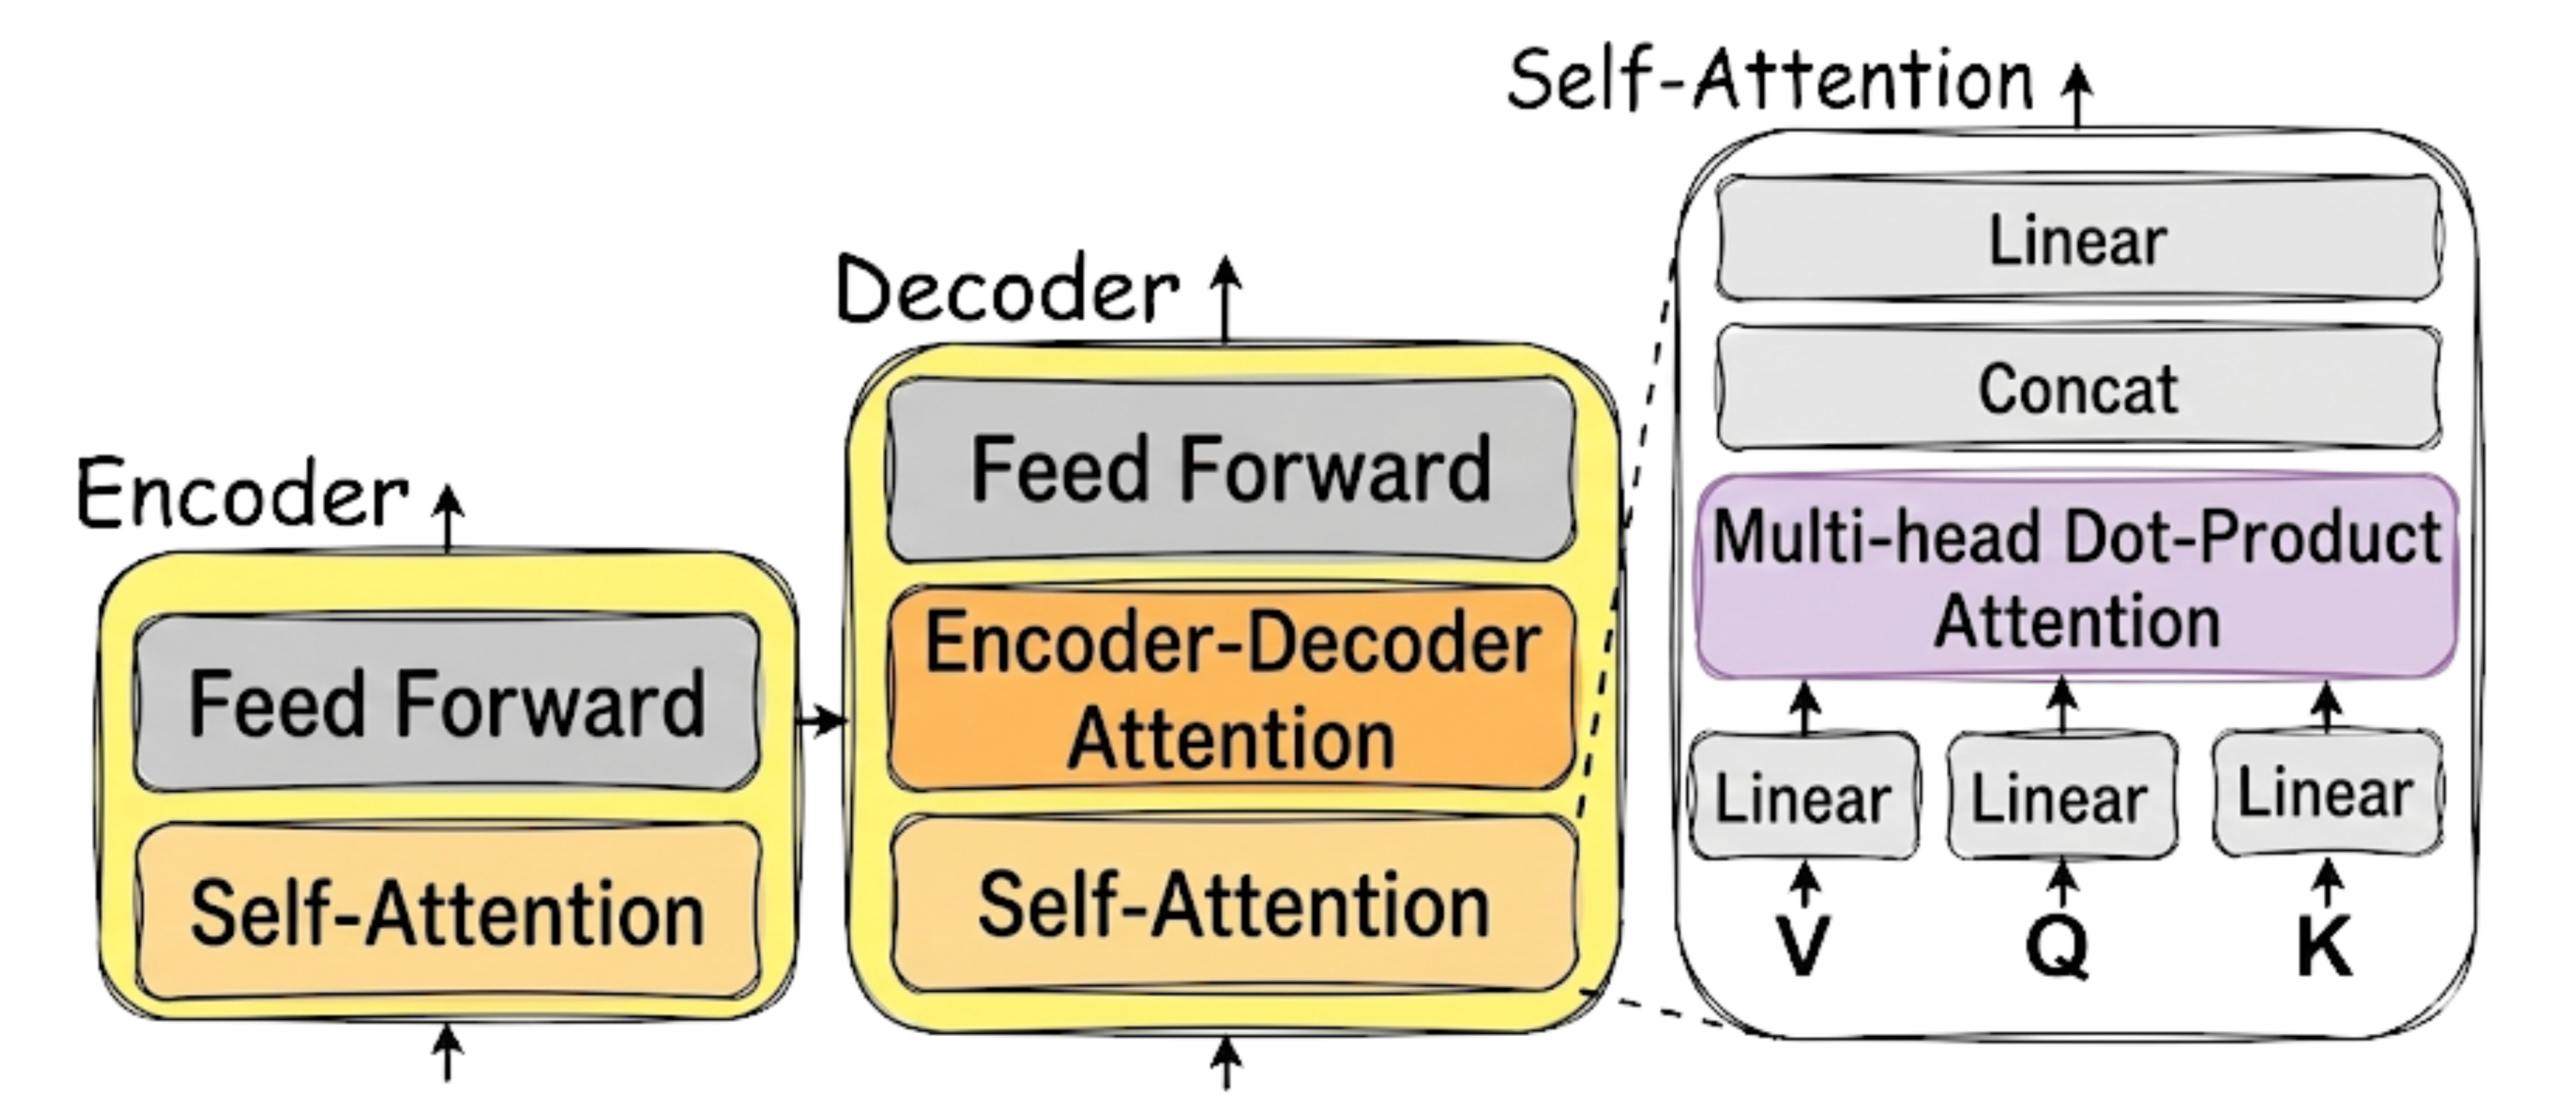
\includegraphics[width=0.8\textwidth]{Gambar/transformer.png}}
	\caption{Ilustrasi \textit{LLM} berbasis \textit{Transformer} dengan mekanisme \textit{self-attention}}
	\label{fig:transformer-arch}
\end{figure}

Perkembangan model bahasa besar telah mengalami perubahan arsitektural yang signifikan. Menurut \cite{devlin2019bertpretrainingdeepbidirectional}, model berbasis \textit{bidirectional} seperti BERT unggul dalam pembelajaran representasi linguistik kontekstual. Sementara itu, menurut \cite{Radford2018ImprovingLU}, model dengan arsitektur \textit{auto-regressive} yang menggunakan \textit{transformer unidirectional} memiliki keunggulan dalam \textit{text generation}. Dengan peningkatan jumlah parameter pada \textit{Large Language Model} dan pelatihan pada dataset yang jauh lebih besar, muncul kemampuan baru yang sebelumnya tidak terprediksi, muncul kemampuan emergen yang meliputi kemampuan belajar dari hanya beberapa contoh (\textit{few-shot learning}) serta melakukan penalaran berantai dengan beberapa langkah (\textit{chain-of-thought reasoning}) \cite{wei2023chainofthoughtpromptingelicitsreasoning}. Meskipun arsitektur \textit{auto-regressive} lebih fleksibel untuk tugas asisten penelitian, model ini memiliki risiko tinggi dalam menghasilkan teks yang fasih namun tidak didukung oleh fakta eksternal.

Model LLM terkini seperti GPT-4 \citep{openai2024gpt4technicalreport} dan Deepseek-R1 \citep{deepseekai2025deepseekr1incentivizingreasoningcapability} menunjukkan performa stabil dalam berbagai pengujian. Mekanisme generasi teksnya didasarkan pada perhitungan probabilitas untuk menentukan token berikutnya dengan probabilitas tertinggi, yang dirumuskan sebagai:

\begin{equation}
y_t = \arg\max_y P_\theta(y_t \mid y_{t-1}, \cdots, y_1, x)
\label{eq:llm-generation}
\end{equation}
di mana \(P_\theta\) melambangkan fungsi probabilitas yang dipelajari oleh model, \(x\) merupakan input teks dari pengguna, dan \(y_1, \cdots, y_t\) adalah token keluaran yang dihasilkan secara berurutan. Bagaimanapun, \text{LLM} tetap menghadapi Tantangan utama seperti halusinasi \cite{Ji_2022}, keterbatasan pengetahuan temporal, serta kesulitan dalam penalaran yang kompleks \cite{bubeck2023sparksartificialgeneralintelligence}. 

Meskipun teknik penyelarasan seperti \textit{Reinforcement Learning from Human Feedback} (RLHF) \citep{ouyang2022traininglanguagemodelsfollow} dan model \textit{open-source} seperti LLaMA \citep{touvron2023llamaopenefficientfoundation} telah mendemokratisasi akses AI, terdapat celah teoretis (\textit{theoretical gap}) di mana model-model ini masih kesulitan mengakses data akademik spesifik yang bersifat \textit{private} atau lokal, seperti data publikasi dosen Infokom UNESA. Ketergantungan LLM pada ingatan parametrik (\textit{parametric memory}) menyebabkan ketidakmampuan dalam memberikan referensi ilmiah yang valid dan terupdate secara \textit{real-time}
		
\subsection{Retrieval-Augmented Generation (RAG)}

\textit{Retrieval-Augmented Generation} (\text{RAG}) merupakan sebuah kerangka kerja yang memungkinkan Model Bahasa Besar untuk mengakses sumber informasi eksternal sebelum memberikan jawaban \citep{lewis2021retrievalaugmentedgenerationknowledgeintensivenlp}. Menurut \cite{Huang_2025}, pendekatan ini secara efektif mengatasi beberapa keterbatasan mendasar \text{LLM}, seperti kecenderungan menghasilkan jawaban yang salah atau mengada-ada (\textit{hallucination}), pengetahuan yang sudah usang, serta kekurangan keahlian dalam domain tertentu. Dengan mendasarkan respons pada dokumen-dokumen yang diambil dari basis pengetahuan, \textit{RAG} memperluas kemampuan \textit{LLM}. Model \textit{LLM }tidak hanya mengandalkan ingatan dari masa pelatihan, tetapi juga dapat mengakses dokumen terbaru secara langsung, sehingga menghasilkan jawaban yang lebih akurat dan dapat dipercaya tanpa perlu melakukan pelatihan ulang yang memakan biaya besar. Saat ini, \text{RAG} telah menjadi solusi di berbagai bidang:

\begin{itemize}
    \item \textbf{Sistem Tanya Jawab Umum (\textit{Open-Domain QA}):} RAG meningkatkan akurasi jawaban dengan mengambil informasi dari sumber luas seperti \textit{Wikipedia} atau kumpulan data khusus seperti halnya Natural Questions dan TriviaQA \citep{joshi2017triviaqalargescaledistantly}.
    
    \item \textbf{Bidang Hukum dan Kesehatan:} RAG digunakan untuk mencari aturan hukum terbaru atau jurnal medis terkini secara cepat[cite: 339]. Hal ini sangat penting untuk memastikan setiap keputusan profesional didasarkan pada bukti yang sah dan referensi yang terpercaya \citep{xiong2024benchmarkingretrievalaugmentedgenerationmedicine}.
    
    \item \textbf{Asisten Virtual dan \textit{Chatbot}:} Dengan RAG, asisten digital menjadi lebih pintar karena mampu menarik data terbaru, seperti laporan keuangan atau berita terkini, dari basis data organisasi maupun internet. Hal ini memungkinkan model memberikan jawaban yang selalu diperbarui dan sesuai konteks kebutuhan pengguna.
\end{itemize}

Dalam perkembangannya, penelitian oleh \cite{gao2024retrievalaugmentedgenerationlargelanguage} mengklasifikasikan evolusi metode \textit{RAG} ke dalam tiga paradigma utama. Pertama, \textbf{Naive RAG} menggunakan pola "\textit{retrieve-read}" sederhana yang mengambil dokumen berdasarkan kesamaan pertanyaan, namun sering kali menghasilkan informasi yang kurang relevan \citep{jiang2025reasoningenhancedhealthcarepredictionsknowledge}. Kedua, \textbf{Advanced RAG} meningkatkan proses pencarian dengan \textit{query expansion} sebelum melakukan pengambilan dan \textit{reranking} dokumen, sehingga data yang diberikan kepada \textit{LLM} menjadi lebih akurat \citep{ma2023queryrewritingretrievalaugmentedlarge}.  Terakhir, \textbf{Modular RAG} menawarkan fleksibilitas melalui modul fungsional yang dapat disesuaikan untuk mengolah data struktural seperti grafik atau tabel, mendukung adaptasi pada beragam tugas \citep{Wang2023KnowledGPTEL}. Alur integrasi dari paradigma-paradigma ini secara visual digambarkan pada \ref{fig:rag-process}.

\begin{figure}[!t]
	\centering
	\makebox[\textwidth][c]{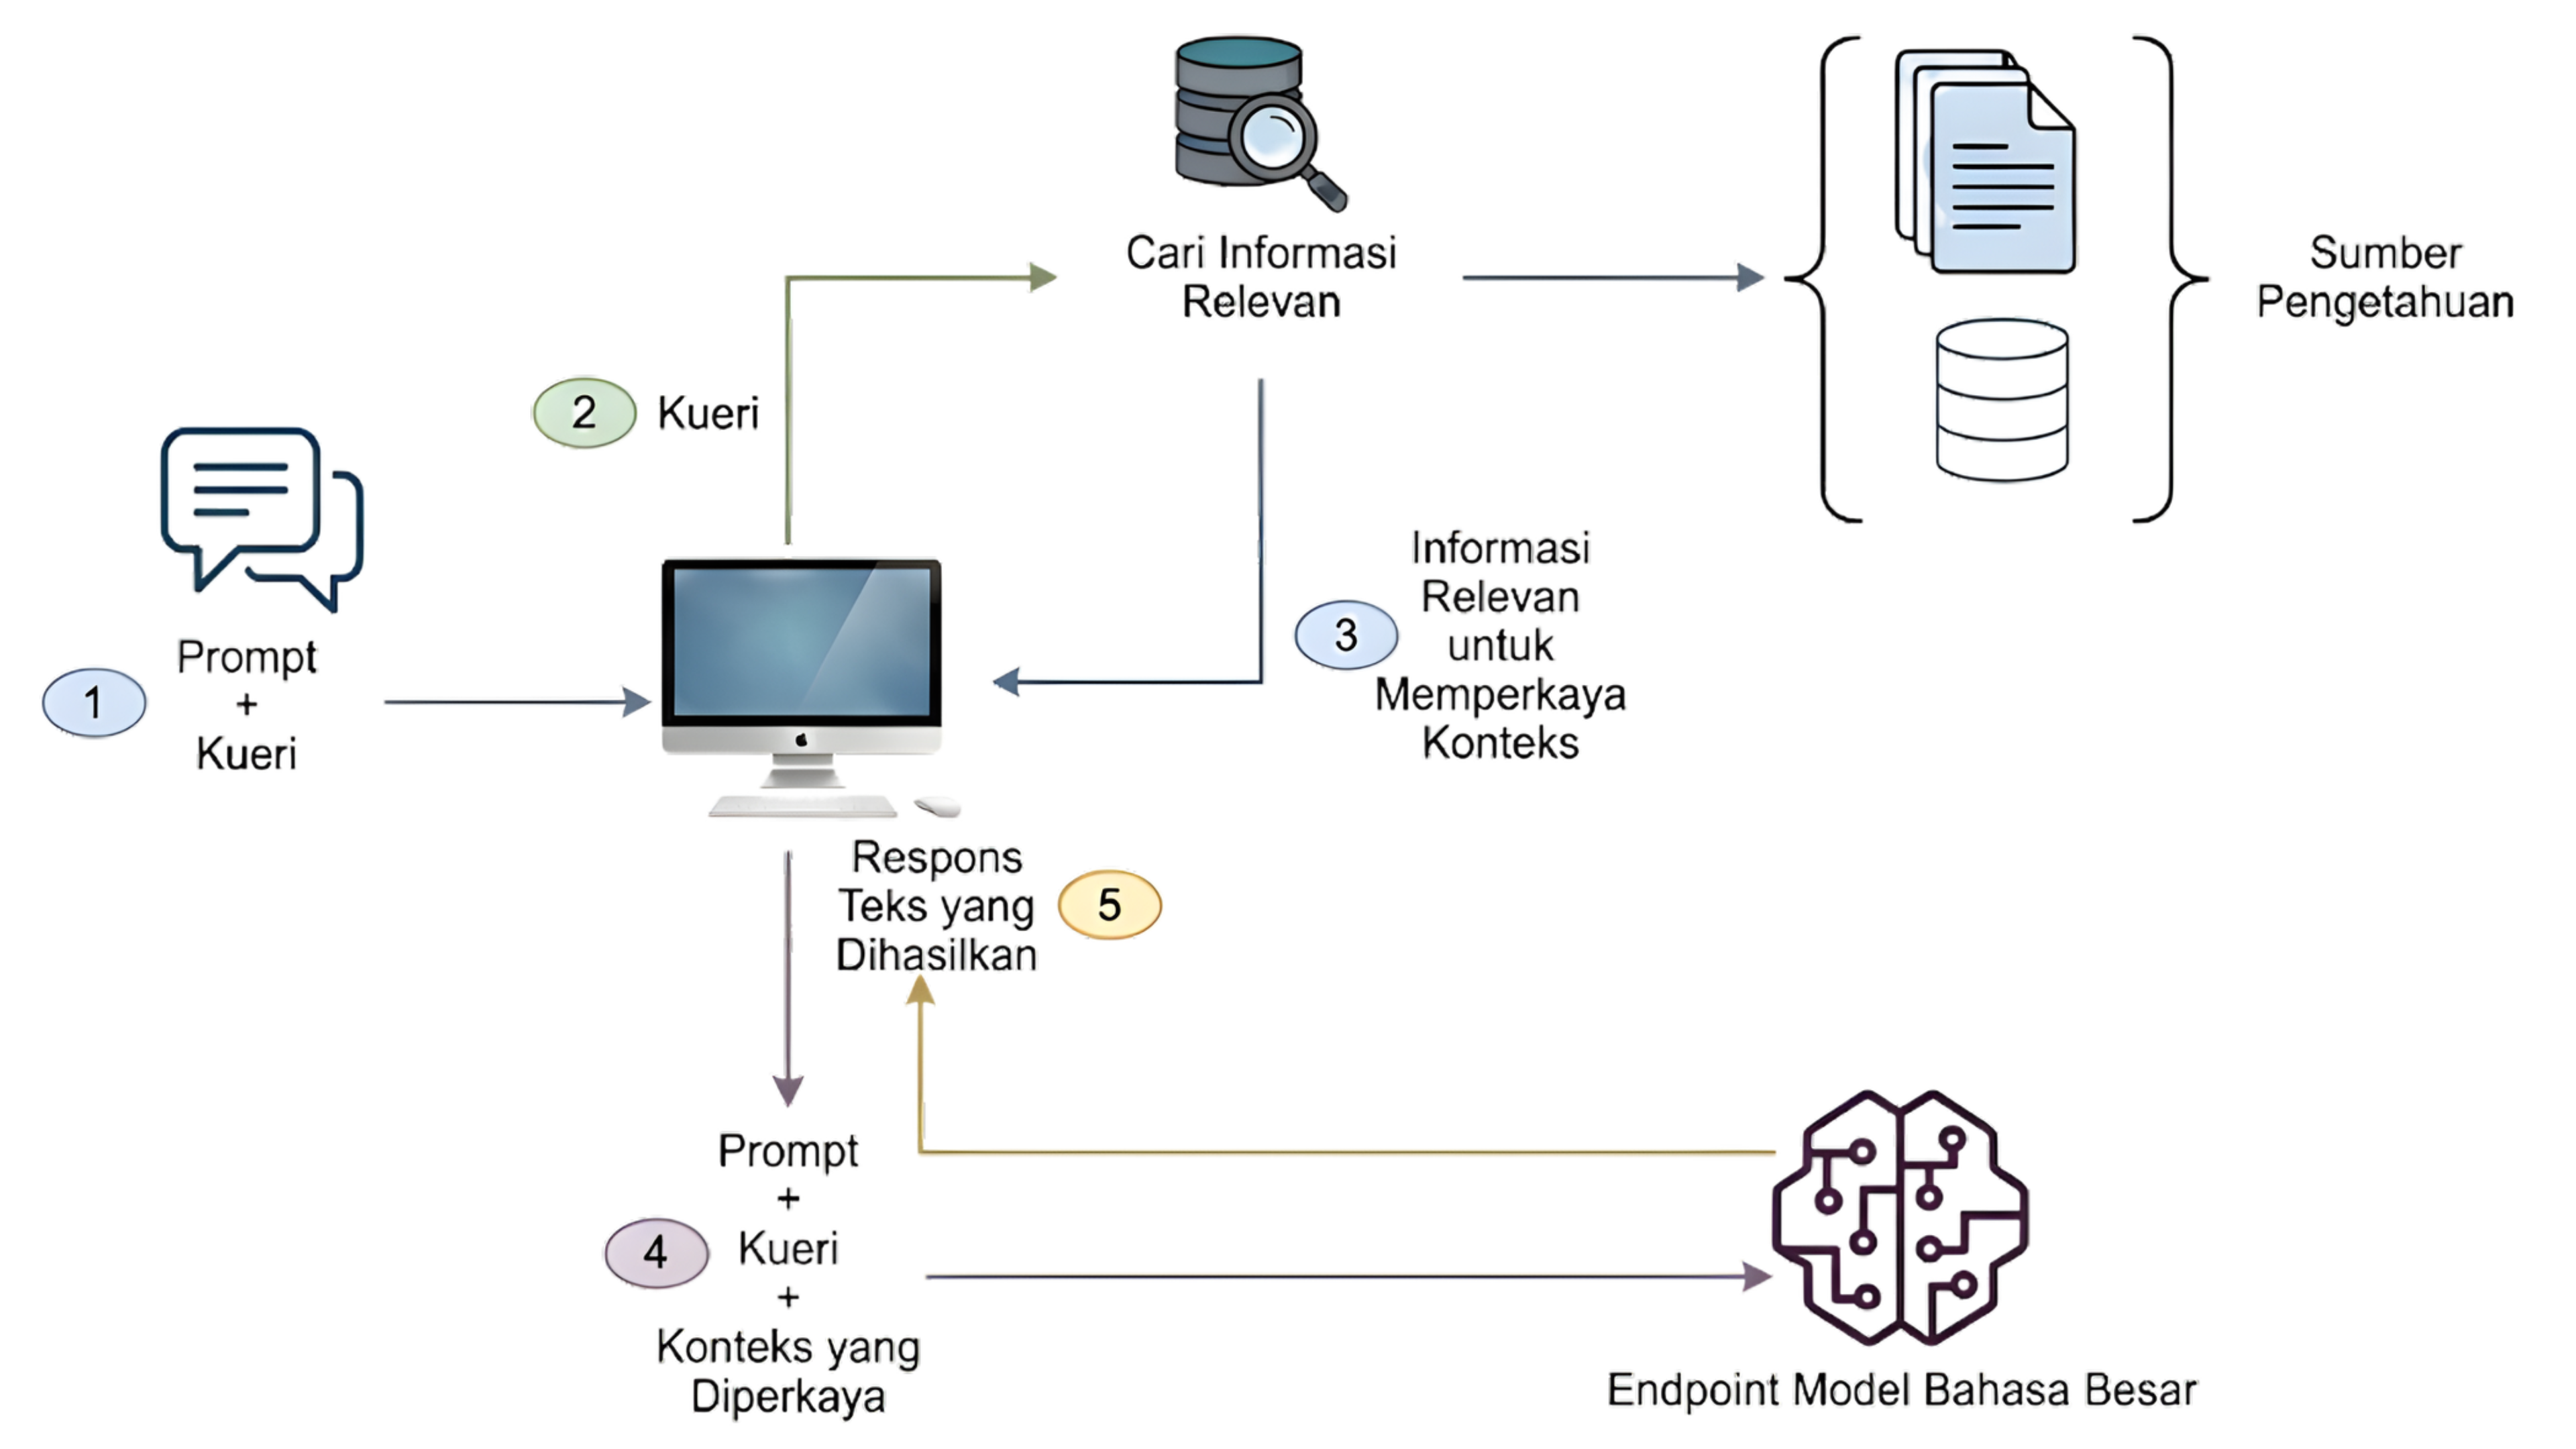
\includegraphics[width=1\textwidth]{Gambar/rag new.png}}
	\caption{Diagram Alur \text{RAG}}
	\label{fig:rag-process}
\end{figure}

Secara definisi, \textit{RAG} adalah proses mengidentifikasi dan mengambil dokumen-dokumen relevan dari sekumpulan dokumen berdasarkan pertanyaan pengguna sebagai konteks untuk \textit{LLM}, atau yang disebut oleh \cite{Hambarde_2023} sebagai \textit{information retrieval}. Penelitian oleh \cite{luan2021sparsedenseattentionalrepresentations} menunjukkan bahwa penggunaan satu metode pencarian untuk \textit{Information Retreival} sering kali gagal menemukan informasi relevan apabila pertanyaan pengguna bersifat kompleks. Penelitian terkini juga menunjukkan bahwa penggunaan satu metode pengambilan informasi kurang efektif. Contohnya, penelitan \cite{luan2021sparsedenseattentionalrepresentations} melakukan pengembangan yang menggabungkan dua pendekatan yaitu pencarian berbasis kata kunci (\textit{sparse retrieval}) dan pencarian berdasarkan makna atau konteks (\textit{dense retrieval}). Kolaborasi ini memastikan sistem tetap akurat meskipun pengguna menggunakan istilah berbeda yang memiliki makna serupa.

Meskipun metode \textit{Hybrid Retrieval} sangat membantu, metode \text{RAG} konvensional tetap masih bergantung pada pencocokan vektor yang ditemukan dan mengabaikan hubungan antar informasi di dalamnya. Di sinilah pentingnya penggunaan \textit{Knowledge Graph} untuk membantu \text{RAG} memahami keterkaitan antar konsep secara lebih menyeluruh. Dalam penelitian ini, \textit{Hybrid Retrieval} diarahkan untuk mengisi kekurangan tersebut dengan mengembangkan sistem \text{RAG} yang tidak hanya hibrida dalam pencarian, tetapi juga diperkuat oleh struktur graf guna mendukung pencarian referensi akademik yang lebih mendalam. 

\subsection{Graph-Based RAG}

\textit{Graph-Based Retrieval-Augmented Generation} (Graph-RAG) merupakan evolusi dari arsitektur RAG konvensional yang menggabungkan kekuatan Model Bahasa Besar dengan struktur data graf untuk menangkap hubungan antar informasi yang kompleks \citep{peng2024graphretrievalaugmentedgenerationsurvey}. Berbeda dengan \text{RAG} konvensional yang biasanya mengambil potongan teks yang tidak terstruktur, Graph-RAG secara khusus mengekstraksi elemen-elemen graf yang relevan, termasuk entitas, relasi, atau bahkan subgraf, dengan tujuan memperkaya konteks pada Model Bahasa Besar (\text{LLM}) \citep{guo2023gpt4graphlargelanguagemodels}. Hal ini sangat essential jika di bawah ke ranah Akademik karena domain akademik memerlukan data terstruktur atua berjejaring.

\begin{figure}[!t]
    \centering
    
\includegraphics[width=1\textwidth]{Gambar/framework graphrag.png}
    \caption{Alur Graph-Based RAG untuk tugas \textit{Question-Answering}
    \citep{peng2024graphretrievalaugmentedgenerationsurvey}}
    \label{fig:graphrag-framework}
\end{figure}

Kerangka kerja \textit{Graph-Based RAG} secara garis besar terbagi menjadi tiga tahapan utama yang saling terintegrasi dalam satu alur kerja, sebagaimana diilustrasikan pada \ref{fig:graphrag-framework}:

\begin{itemize}
    \item \textbf{Graph-Based Indexing (G-Indexing):} Merupakan tahap pembangunan basis data graf terstruktur yang berfungsi sebagai sumber pengetahuan. Proses ini mengorganisir entitas (\textit{nodes}) dan relasi (\textit{edges}) sedemikian rupa untuk mengoptimalkan pencarian. Data graf ini dapat berasal dari sumber terbuka seperti Wikidata \cite{wikidata} atau dibangun secara mandiri dari kumpulan dokumen akademik tertentu. Indeksasi adalah tahap paling krusial karena menentukan seberapa detail informasi yang dapat diambil nantinya.
    
    \item \textbf{Graph-Guided Retrieval (G-Retrieval):} Alih-alih mengambil potongan teks, sistem bertujuan mengambil elemen graf yang paling relevan, seperti pasangan subjek-predikat-objek (\textit{triples}), jalur hubungan (\textit{paths}), atau subgraf utuh. Metode pengambilannya bisa melalui algoritma penelusuran graf tradisional, pencarian kesamaan semantik, maupun model berbasis Jaringan Saraf Graf (\textit{GNN}).
    
    \item \textbf{Graph-Enhanced Generation (G-Generation):} Pada tahap akhir, data graf yang diambil diintegrasikan ke dalam proses pembuatan jawaban. Struktur graf ini dapat diubah menjadi teks naratif atau diproses langsung oleh model \textit{transformer} yang peka terhadap struktur graf agar menghasilkan respons yang koheren, informatif, dan valid.
\end{itemize}

Untuk memberikan landasan teoretis bagi tahapan-tahapan praktis yang telah dijelaskan sebelumnya, berikut adalah formulasi matematis yang mendasari kerangka kerja Graph-RAG. Secara teoretis, tujuan utama dari \textit{Graph-RAG} adalah menemukan jawaban terbaik ($a^*$) untuk sebuah pertanyaan ($q$) berdasarkan Graf Pengetahuan ($\mathcal{G}$). Hal ini dirumuskan dalam Persamaan \ref{eq:graphrag_goal}:

\begin{equation}
	a^* = \operatorname*{arg\,max}_{a \in A} p(a|q, \mathcal{G})
	\label{eq:graphrag_goal}
\end{equation}
di mana \(A\) merepresentasikan himpunan seluruh kemungkinan respons yang dapat dihasilkan. Untuk mencapai tujuan tersebut, distribusi probabilitas target \(p(a \mid q, \mathcal{G})\) dimodelkan melalui kolaborasi dua komponen utama yaitu model \textit{graph retriever} \(p_\theta(G \mid q, \mathcal{G})\) dan model \textit{answer generator} \(p_\phi(a \mid q, G)\), di mana \(\theta\) dan \(\phi\) adalah parameter yang dapat dilatih.

Untuk mencapai hasil tersebut secara efisien tanpa harus menelusuri seluruh isi graf yang sangat besar, sistem menggunakan pendekatan perkiraan dengan hanya memilih subgraf yang paling relevan ($G^*$). Hubungan antara model pencari (\textit{retriever}) dan (\textit{generator}) ini dapat didekomposisi sebagai berikut:

\begin{equation}
\begin{split}
	p(a \mid q, \mathcal{G}) &= \sum_{G \subseteq \mathcal{G}} p_\phi(a \mid q, G)\, p_\theta(G \mid q, \mathcal{G}) \\
    &\approx p_\phi(a \mid q, G^*)\, p_\theta(G^* \mid q, \mathcal{G})
\end{split}
\label{eq:graphrag_decomposition_approx}
\end{equation}
Di sini, $p_\theta$ mewakili parameter model \textit{retriever} yang mencari subgraf relevan, sementara $p_\phi$ adalah model \textit{generator} yang menyusun jawaban berdasarkan subgraf tersebut.

Perkembangan \textit{Graph-based RAG} telah melahirkan berbagai pendekatan dengan kelebihan dan kekurangannya masing-masing, pendekatan berbasis komunitas (\textit{Community-based}) pertama kali dipelopori oleh \cite{edge2025localglobalgraphrag}, metode ini menggunakan \textit{LLM} untuk membangun\textit{Knowledge Graph} (KG) dan algoritma deteksi komunitas untuk membagi graf menjadi kelompok-kelompok informasi. Namun, metode ini memiliki tantangan pada biaya komputasi yang tinggi, masalah skalabilitas saat data bertambah, serta risiko masuknya informasi yang tidak relevan dari laporan komunitas jika terlalu luas. Sebagai perbaikan, model seperti \textit{LightRAG} memperkenalkan pengambilan dua tingkat menggunakan kata kunci lokal dan global \citep{guo2025lightragsimplefastretrievalaugmented}. Teknik ini secara signifikan mengurangi beban penyimpanan dan mempercepat pencarian tetapi kurang fleksibel untuk jenis teks seperti domain akademik dan berisiko melewatkan hubungan antar entitas jika tidak disebutkan secara eksplisit.

Pengembangan dalam bidang ini masih terbuka lebar. Metode berbasis komunitas \textit{Community-based} \citep{edge2025localglobalgraphrag} terlalu boros sumber daya, metode berbasis aturan \textit{R} \citep{hu2025cgragresearchquestionanswering} sulit diterapkan secara luas, dan metode berbasis kata kunci \textit{Keyword-based} \citep{guo2025lightragsimplefastretrievalaugmented} terkadang masih terkendala pada kualitas hasil akhir jika tidak di sebutkan secara eksplisit. Berdasarkan observasi tersebut, masih diperlukan sistem \textit{Information Retrieval} dengan pendekatan \textit{hybrid retrieval} yang mampu mengombinasikan berbagai metode pengambilan informasi, seperti pengambilan konvensional\textit{semantic retreival} (Vektor) dikombinasikan \textit{Structured Retreival} (Graf). Pendekatan ini bertujuan untuk menyeimbangkan efisiensi komputasi dengan akurasi pencarian, sehingga sistem dapat menyajikan referensi ilmiah yang relevan dan mendalam tanpa terbebani biaya operasional yang besar.